\section{Probability}

\begin{defn}[Geometric Distribution]
$N$ is geometrically distributed with parameter $p \in (0,1]$ if $N$ is a non-negative integer random variable with probability mass function
$$
P(N = n) = (1 - p)^{n - 1} p
$$
for $n \in \{1,2,\ldots\}$.

Unless otherwise specified, in this paper a geometric distribution is assumed to be supported on $\{1,2,\ldots\}$.
\end{defn}

\begin{defn}[Exponential Distribution]
Let $X$ be a random variable.
If $X$ has a probability density function
$$
f(x; \lambda) = \begin{cases}
    \lambda e^{-\lambda x} & x > 0\\
    0 & x \leq 0
    \end{cases}
$$
then we say that $X$ is exponentially distributed with rate $\lambda$, denoted as $X \sim \exp(\lambda)$.
\end{defn}

\begin{defn}[Gamma Distribution]
Let $X$ be a random variable.
If $X$ has a probability density function
$$
f(x; \alpha, \beta) = \frac{1}{\Gamma(\alpha)} \beta^\alpha x^{\alpha - 1} e^{-\beta x} \quad x > 0, \alpha, \beta > 0
$$
where
$$
\Gamma(\alpha) = \begin{cases}
    (\alpha + 1) ! & \alpha \in \{1,2,\ldots\}\\
    \int_{0}^\infty x^{\alpha - 1} e^{-\alpha} ~dx & \alpha \in (0, \infty)
\end{cases}
$$
then we say that $X$ has a gamma distribution with a shape parameter $\alpha \in (0, \infty)$ and rate parameter $\beta \in (0, \infty)$.
\end{defn}

\begin{theorem}\label{thm:exp_x_less_y}
Let $X \sim \exp(\alpha)$ and $Y \sim \exp(\beta)$ be independent random variables.
Then
$$
P(X < Y) = \frac{\alpha}{\alpha + \beta}
$$
\end{theorem}

\begin{proof}
\begin{align*}
    P(X < Y) &= \int_0^\infty P(X < y | Y = y) f_Y(y) dy\\
    &= \int_0^\infty (1 - e^{-\alpha y}) \beta e^{-\beta y} dy\\
    &= \beta \int_0^\infty \left( e^{-\beta y} - e^{-(\alpha + \beta) y}\right) dy\\
    &= \beta \left(\frac{1}{\beta} - \frac{1}{\alpha + \beta}\right)\\
    &= \frac{\alpha}{\alpha + \beta}
\end{align*}
\end{proof}

\begin{theorem}\label{thm:exp_t_cond}
Let $X$ be exponentially distributed with parameter $\alpha$ (denoted $X \sim \exp(\alpha)$) and $Y \sim \exp(\beta)$ be independent random variables with $T = \min(X,Y)$
Then $T \sim \exp(\alpha + \beta)$.
\end{theorem}

\begin{proof}
\begin{align*}
    P(\min(X,Y) > z) &= P(X > z, Y > z)\\
    &= P(X > z) P(Y > z)\\
    &= e^{-\alpha z} e^{-\beta z}\\
    &= e^{-(\alpha + \beta) z}
\end{align*}
So $\min(X,Y) = T \sim \exp(\alpha + \beta)$
\end{proof}

\begin{theorem} \label{thm:exp_scaling}
Let $X \sim \exp(\lambda)$ and $c > 0$ be a constant.
Then $cX \sim \exp(\lambda/c)$.
\end{theorem}

\begin{proof}
$$
    P(cX > y) = P(X > y/c) = e^{-y (\lambda/c)} \quad y > 0
$$
So $cX \sim \exp(\lambda/c)$
\end{proof}

\subsection{Generating functions and Characteristic Functions}

\begin{defn}[Probability generating function]
The probability generating function of a discrete random variable $X \in \{0,1,2, \ldots\}$ is defined as
$$
G_X(z) = E[z^X] = \sum_{i = 0}^\infty z^i P(X = i)
$$
for all $z \in \R$ in which the sum converges.
\end{defn}

\begin{note}
For a discrete non-negative integer-valued random variable $X$,
\begin{itemize}
    \item $G_X(0) = P(X = 0)$ since we define $0^0 = 1$
    \item $G_X(1) = 1$
\end{itemize}
\end{note}

\begin{defn}[Characteristic function]
The characteristic function of a random variable $X$ is the function $\varphi_X : \R \to \mathbb C$ defined as
$$
\varphi_X(t) = E[e^{itX}]
$$

where $i = \sqrt{-1}$.
\end{defn}

\begin{remark}
Some properties about the characteristic function
\begin{itemize}
    \item $\varphi_X(0) = 1$
    \item If the $k$th moment exists for $X$ then $\varphi_X$ is $k$ times differentiable and $E[X^k] = \varphi_{X}^{(k)}(0) i^{-k}$
\end{itemize}
\end{remark}

\begin{theorem}[Moments from generating function]
Let $X$ be a discrete random variable on the non-negative integers and $G_X(z)$ be its probability generating function
\begin{itemize}
    \item $E[X] = G'(1)$
    \item $E[X (X - 1) \cdots (X - k + 1)] = G^{(k)}(1)$
\end{itemize}
provided the derivatives exist.
\end{theorem}

\begin{proof}
See \cite{grimmett2001}
\end{proof}

\begin{theorem}
If $X$ and $Y$ are independent non-negative integer random variables then
$$
G_{X + Y}(z) = G_X(z) G_Y(z)
$$
for $z \in \R$ in which the sums converge.
\end{theorem}

\begin{proof}
See \cite{grimmett2001} or \cite{Ross_SP_95}
\end{proof}

\begin{theorem}
For any independent random variables $X$ and $Y$,
$$
\varphi_{X + Y}(t) = \varphi_X(t) \varphi_Y(t)
$$
for all $t \in \R$.
\end{theorem}

\begin{proof}
See \cite{grimmett2001}
\end{proof}

\begin{theorem}\label{thm:generating_random_sum}
Let $X_1, X_2, \ldots$ be i.i.d random variables with common probability generating function $G_X(z)$.
Let $N$ be another non-negative integer random variable, independent of the sequence $(X_n)$ and $G_N(z) = E[z^N]$ be the probability generating functions for $N$.
Let $S = \sum_{i = 1}^N X_i$.
Then,
$$
G_S(z) = G_N(G_X(z))
$$
\end{theorem}

\begin{proof}
\begin{align*}
    G_X(z) &= E[ z^S ]\\
    &= E[ E[ z^{\sum_{i = 1}^N X_i} | N ]]\\
    &= E \left[ \prod_{i = 1}^N E[z^{X_i}] \right] && \text{by independence}\\
    &= E[ G_X(z)^N]\\
    &= G_N(G_X(z))
\end{align*}
\end{proof}

\begin{theorem}\label{thm:char_func_random_sum}
Let $X_1, X_2, \ldots$ be i.i.d random variables with common characteristic function $\varphi_X(t)$.
Let $N$ be a non-negative integer random variable, independent of the sequence $(X_n)$.
Let $G_N(z) = E[z^N]$ be the probability generating function for $N$.
Let $S = \sum_{i = 1}^N X_i$.
Then,
$$
\varphi_S(t) = E[\varphi_X(t)^N] = G_N(\varphi_X(t))
$$
\end{theorem}

\begin{proof}
\begin{align*}
    \varphi_S(t) &= E[ \exp(it \sum_{i = 1}^N X_i) ]\\
    &= E[ E[ \exp(it \sum_{i = 1}^N X_i) | N ]]\\
    &= E \left[ \prod_{i = 1}^N E[\exp(it X_i)] \right] && \text{by independence}\\
    &= E[\varphi_X(t)^N]\\
    &= G_N(\varphi_X(t))
\end{align*}
\end{proof}

\begin{defn}[Finite mixture]
Let $X_1,\ldots, X_n$ be random variables.
We first sample from the random variables according to weights $\alpha = (\alpha_1, \ldots, \alpha_n)$ with $\sum_i \alpha_i = 1$ and $\alpha_i \geq 0$.
Then choose a realization from the selected random variable.
This new random variable $X$ is called a \textbf{mixture} of $X_1,\ldots, X_n$.

Let $F_1, \ldots, F_n$ be the corresponding cumulative distribution functions (CDF) of $X_1, \ldots, X_n$ and $f_1, \ldots, f_n$ the probability density functions (if they exist).
Then the CDF of $X$ is defined as
$$
F(x) = \sum_{j = 1}^n \alpha_j F_j(x)
$$
and the PDF is defined as
$$
f(x) = \sum_{j = 1}^n \alpha_j f_j(x)
$$
\end{defn}

\begin{defn}[Convolution]
Let $f$ and $g$ be functions. Then, the convolution of $f$ and $g$, denoted $f * g,$ is defined as
$$
(f * g)(z) = \int_{-\infty}^\infty f(t) g(z - t)~dt =  \int_{-\infty}^\infty f(z - t) g(t)~dt
$$
\end{defn}

\begin{theorem}
Let $X$ and $Y$ be independent absolutely continuous random variables with density functions $f$ and $g$.

Then the distribution of $Z = X + Y$ has a density function
$$
h(z) = (f * g)(z)
$$
where $*$ is convolution.

If $X$ and $Y$ are independent integer random variables, then
$$
P(Z = z) = \sum_{k = -\infty}^\infty P(X = k) P(Y = z - k)
$$
\end{theorem}

% \begin{defn}[Hazard Function]\cite{ross1996stochastic}
% Let $T$ random variable with PDF $f(t)$ and CDF $F(t)$ and the survival function $S(t) = 1 - F(t)$.
% Then the hazard function is defined as
% $$
% h(t) = \frac{f(t)}{S(t)}
% $$

% If $T$ represents some event, then the hazard function $h(t)$ is the probability of an event occurring in $t + dt$ given that no event has occurred until time $t$. 
% \end{defn}

\subsection{Random Sums}

\begin{theorem} \label{thm:geom_sum_exp}
Let $N$ be geometrically distributed ($N \in \{1,2,\ldots\})$ with probability of success $p$ and $X_1,X_2,\ldots$ i.i.d and independent of $N$ with each $X_i$ exponentially distributed with rate $\lambda$.
Then,
$$
S = \sum_{i = i}^N X_i
$$
has an exponential distribution with rate $p \lambda$.
\end{theorem}

\begin{proof}
Let $G_N(z)$ be the probability generating function of $N$ and $\varphi_X(t)$ be the characteristic function of each $X_i$.
It is easy to show that
\begin{align*}
    G_N(z) &= \frac{pz}{1 - (1 - p)z}\\
    \varphi_X(t) &= \frac{\lambda}{\lambda - it}
\end{align*}
Then by Theorem \ref{thm:char_func_random_sum},
\begin{align*}
    \varphi_S(t) &= G_N(\varphi_X(t))\\
    &= \frac{
        p \left( \frac{\lambda}{\lambda - it} \right)
        } {
        1 - (1 - p) \frac{\lambda}{\lambda - it}
        }\\
    &= \frac{
        p \lambda
    } {
        \lambda - it - \lambda + p \lambda
    }\\
    &= \frac{
        p \lambda
    } {
        p \lambda - it
    }
\end{align*}
which is the characteristic function of the exponential distribution with rate $p \lambda$.
\end{proof}

\begin{theorem}[Wald's equation]\label{thm:random_sum_ev}
Let $X_1, X_2, \ldots$ be sequence of i.i.d random variables with finite expectation and $N$ a non-negative integer random variable independent of the sequence $(X_n)$, also with finite expectation.
Let $S = \sum_{i = 1}^N X_i$.
Then,
$$
E[ S ] = E\left[\sum_{i = 1}^N X_i\right] = E[X] E[N]
$$
\end{theorem}

\begin{proof}
Let $G_N(z)$  be the probability generating function for $N$ and $\varphi_X(t)$ be the characteristic function for each $X_i$.
By Theorem \ref{thm:char_func_random_sum}, we have that the characteristic function of $S$ is $\varphi_S(t) = G_N(\varphi_X(t))$.
Hence,
$$
\varphi'_S(t) = G'_N(\varphi_X(t)) \cdot \varphi'_X(t)
$$
It follows that
\begin{align*}
    E[S] &= \varphi'_S(1) i^{-1}\\
    &=  G'_N(\varphi_X(0)) \cdot \varphi'_X(0) i^{-1}\\
    &= G'_N(1) [\varphi'_X(0) i^{-1}]   \\
    &= E[N] E[X]
\end{align*}

% The not as elegant way.
%\begin{align*}
%    E\left[ \sum_{i = 1}^N X_i \right] &= E\left[ E\left[ \sum_{i = 1}^N X_i | N\right] \right]\\
%    &= \sum_{n = 1}^\infty E\left[ \sum_{i = 1}^n X_i \right] P(N = n) && N, (X_t) \text{ indep.}\\
%    &= \sum_{n = 1}^\infty \sum_{i = 1}^n E\left[ X_i \right] P(N = n)\\
%    &= E\left[ X_i \right] \sum_{n = 1}^\infty n \cdot P(N = n)\\
%    &= E[X_i] E[N]
%\end{align*}
\end{proof}

\begin{theorem} \label{thm:random_sum_var}
Let $X_1, X_2, \ldots$ be i.i.d random variables with finite variance and $N$ a non-negative integer random variable with finite variance, independent of ($X_n$).
Then,
$$
\Var\left( \sum_{i = 1}^N X_i \right) = E[N]\Var(X) + (E[X])^2 \Var(N)
$$
\end{theorem}

\begin{proof}
See \cite{Ross97}
\end{proof}

The following is analogous to Theorem \ref{thm:geom_sum_exp} but for discrete geometric sums.

\begin{theorem}\label{thm:geom_sum_geom} (\cite{Nelson1995})
Let $X_1, X_2, \ldots$ be i.i.d geometric random variables ($X_i \in \{1,2,\ldots\})$, with parameters $p$ and $N$ a geometric random variable ($N \in \{1,2,\ldots\})$ with parameter $\alpha$, independent of the sequence $(X_n)$.
Then,
$$
S = \sum_{i = 1}^N X_i
$$
is geometrically distributed with parameter $\alpha p$.
\end{theorem}

\begin{proof}
The probability generating functions for $N$ and each $X_i$ are
\begin{align*}
    G_X(z) &= \frac{p z}{1 - (1 - p)z}\\
    G_{N}(z) &= \frac{\alpha z}{1 - (1 - \alpha)z}
\end{align*}

It follows that
\begin{align*}
    G_S(z) &= G_N(G_X(z))\\
    &= \frac{
    \alpha \left( \frac{p z}{1 - (1 - p)z} \right)
    }{
        1 - (1 - \alpha) \left( \frac{p z}{1 - (1 - p)z} \right)
    }\\
    &= \frac{
        \alpha p z
    }{
        1 - z + pz - pz + \alpha p z
    } \\
    &= \frac{
        \alpha p z
    }{
        1 - (1 - \alpha p) z
    }
\end{align*}
So $S$ is geometrically distributed with parameter $\alpha p$
\end{proof}

\subsection{Convergence}

\begin{defn}[Weak convergence]
A sequence of probability measures $(\mu_n)$ \textbf{converges weakly} to $\mu$ (notated as $\mu_n \Rightarrow \mu$) if
$$
\lim_{n \to \infty} \int f d\mu_n = \int f d\mu
$$
for all bounded and continuous functions $f$.
If $F_n$ and $F$ are the CDFs of $\mu_n$ and $\mu$ then this is equivalent to
$$
\lim_{n \to \infty} F_n(x) = F(x)
$$
for all $x \in \R$ that are continuous for $F$.
\end{defn}

% \begin{theorem}
% $X_n \Rightarrow X$ iff $E[g(X_n)] \to E[g(X)]$ for all continuous and bounded functions $g$.
% \end{theorem}

\begin{theorem}[Convergence together lemma] \label{thm:conv_together_lemma}
If $X_n \Rightarrow X$ and $Y_n \Rightarrow c$, where $c$ is a constant, then $X_n + Y_n \Rightarrow X + c$.
\end{theorem}

\section{Stochastic Processes}

\subsection{Markov Chains}

\begin{defn}[Discrete Markov chain] \cite{schapira2017}
Let $\{X_n : n \geq 0\}$ be a stochastic process with a finite or countable state space $S$.
Each $X_n$ is a discrete random variable with $X_n \in S$.
Let $\mathscr{F}_n = \sigma\{X_0, X_1, \ldots, X_n\}$ which is the $\sigma$-algebra generated by the process up to time $n$.
The process $(X_n)$ is a discrete-time Markov chain if
$$
P(X_{n + 1} \in B | \mathscr{F}_n) = P(X_{n + 1} \in B | X_n)
$$
for each $B \subset S$.
%$$
%P(X_{n + 1} = y | X_n = x, X_{n - 1} = x_{n - 1}, \ldots, X_0 = x_0) = P(X_{n + 1} = y | X_n = x)
%$$
%for all $n \geq 1$ and $y, x, x_{n-1}, \ldots, x_0 \in S$.
\end{defn}

\begin{defn}[Homogeneous Markov Chain]\cite{grimmett2001}
We say that a discrete-time Markov chain $(X_n)$ with state space $S$ is \textbf{time homogeneous} if
$$
P(X_{n + 1} = j | X_n = i) = P(X_{1} = j | X_0 = i) = \mathbf{P}(i,j) = p_{ij}
$$
where $\mathbf{P} = (p_{ij})$ is the $|S| \times |S|$ matrix of transition probabilities
$$
p_{ij} = P(X_{n + 1} = i | X_n = j)
$$

All Markov chains are assumed to be time homogeneous in this thesis unless stated otherwise.
\end{defn}

\begin{remark}
Since for a fixed $i$, $P(i, \cdot)$ is a probability measure then we have that
\begin{itemize}
    \item $p_{ij} \geq 0$ for all $i,j$
    \item $\mathbf{P}$ row sums equal one
    $$
    \sum_{j \in S} p_{ij} = 1 \quad \text{for each } i \in S
    $$
\end{itemize}
\end{remark}

\begin{defn}[Continuous-time Markov chain] \cite{schapira2017}
Let $(X_t) = \{X(t) : t \in \mathbb T\}$, where $\mathbb T$ is some index set (generally $\mathbb T = [0, \infty)$ representing time), be a stochastic process with countable state space $S$.
Let $(\mathscr{F}_t)$ be the natural filtration of $(X_t)$, i.e., $\mathscr{F}_t = \sigma\{ X_s : s \leq t \}$.
The process $(X_t)$ is a continuous-time Markov chain (CTMC) if
$$
P(X_{t} \in B | \mathscr{F}_s) = P(X_{t} \in B | X_s)
$$
for all $s < t$ and $B \subset S$.

%Then $(X_t)$ is a continuous-time Markov chain if
%$$
%P(X(t_n) = j | X(t_{n - 1}) = i_{n-1}, \ldots, X(t_1) = i_{1}) %= P(X(t_n) = j | X(t_{n - 1}) = i_{n - 1})
%$$
%for all $t_1, \ldots, t_n \in \mathbb T$, with $t_1 < \cdots < t_n$.
\end{defn}

\begin{defn}
A function $f$ is $o(h)$ as $h$ goes to 0 if 
$$
\lim_{h \to 0} \frac{f(h)}{h} = 0
$$
\end{defn}

\begin{defn}[Infinitesimal generator matrix]
The \textbf{infinitesimal generator matrix} (or \textbf{transition rate matrix}) $Q$, of a continuous-time Markov chain $(X_t)$ with countable state space $S$, is an $|S| \times |S|$ matrix.
The element $q_{ij}$ of $Q$ denotes the rate departing from i and arriving in state j.
The diagonal is defined as $q_{ii} = - \sum_{j \not = i} q_{ij}$.
Each $i \not = j, q_{ij} \geq 0$ and the rows sum to zero: $\sum_{j} q_{ij} = 0$ for each $i$.

Assuming the chain is in state $i$ at time $t$, the probability of moving to state $j$ in time $h$ for $h \to 0$ is given by
$$
P(X_{t + h} = j | X_{t} = i) = \begin{cases}
    i \not = j & q_{ij} h + o(h)\\
    i = j & 1 + q_{ii} h + o(h)
\end{cases}
$$
\end{defn}

\begin{defn}[Embedded Markov Chain]
Let $(X_t)$ be a continuous-time Markov chain with infinitesimal generator matrix $Q$ and $Y_n$ be the position of the $n$th jump of the process $(X_t)$ with $Y_0$ the initial state of the chain $(X_t)$.
This discrete-time Markov chain $(Y_n)$ is called the \textbf{embedded} (discrete) Markov chain of the process $(X_t)$.
\end{defn}

\begin{defn}[Transient and Recurrent States] \cite{grimmett2001}
Assume we have a Markov chain with state space $S$.
A state $i \in S$ is transient if
$$
P(X_n = i \text{ for some } n \geq 1 | X_0 = i) < 1
$$
and recurrent if
$$
P(X_n = i \text{ for some } n \geq 1 | X_0 = i) = 1
$$
\end{defn}

\begin{defn}[Absorbing State] \cite{grinstead2003}
Let $(X_n)$ be a discrete-time Markov chain.
A state $x \in \Omega$ is absorbing if and only if $P(x,x) = 1$.

If $(X_t)$ is a continuous-time Markov chain then $i \in \Omega$ is absorbing if and only if $Q(x,x) = 0$.
\end{defn}

\begin{defn}[Absorbing Markov Chain] \cite{grinstead2003}
A Markov chain is absorbing if there is at least one absorbing state and it is possible to reach an absorbing state in a finite number of steps from any state.
\end{defn}

\begin{defn}[Canonical Form] \cite{grinstead2003}
Assume we have an absorbing discrete time Markov chain with $r$ absorbing states and $t$ transient states and  transition matrix $P$.
The canonical form of the transition matrix is
\begin{equation}
    P = \begin{pmatrix}
        B & R\\
        0 & I_{r}
    \end{pmatrix}
\end{equation}

where $B$ is an $t \times t$ matrix, $R$ is an $t \times r$ matrix and $I_{r}$ is the $r \times r$ identity matrix and $0$ is the $r \times t$ matrix of all 0's.
The first $t$ states are transient and the last $r$ states are absorbing.
\end{defn}

\begin{theorem}\label{thm:visits_geom}
Let $(X_n)$ be a discrete-time Markov chain with countable state space $S$.
The number of visits to each state is geometrically distributed, with parameter equal to the probability of never returning back to the state.
\end{theorem}

\begin{theorem} \label{thm:fund_exp} \cite{grinstead2003}
Assume that we have an absorbing Markov chain.
Let $B$ be the  $t \times t$ matrix of transient states from the canonical form.
Let $N$ be a matrix with the same dimensions as $B$.
$N_{ij}$ is the expected number of times the chain is in state j when starting in state i for transient states $i$ and $j$. Then,
\begin{equation}
    N = I + B + B^2 + \cdots = (I - B)^{-1}
\end{equation}
\end{theorem}

\begin{proof}
See \cite{grinstead2003}
\end{proof}

\begin{theorem}\label{thm:mc_projection} \cite{LevinPeresWilmer2006}
Let $(X_n)$ be a discrete-time Markov chain with state space $\Omega$ and transition matrix $P$.
Let $\sim$ be an equivalence relation on $\Omega$ and denote the equivalences classes as $\Omega' = \{[x]: x \in \Omega\}$.

If $x \sim x'$ implies that $P(x,[y]) = P(x', [y])$ (where $P(x,A)$ is probability that the chain moves in one step to one of the states $y \in A$ from $x$) then $([X_n])$  is a Markov chain.
The state space is the equivalence classes $\Omega'$ and transition matrix $P'$ defined as $P'([x],[y]) := P(x, [y])$.

We call this new Markov chain $([X_n])$ a projection of $(X_n)$ and say that we projected $(X_n)$ onto $([X_n])$.
\end{theorem}

\begin{theorem}\label{thm:x_N_indep}
Assume that we have a continuous-time Markov chain with an embedded discrete-time Markov chain $(Y_n)$.
Let $U_i$ be the waiting time in state $Y_i$.
The sequence of holding times $(U_n)$ is conditionally independent given the sequence of states $(Y_n)$.

Also, each $U_i | (Y_n) \sim \exp(Q(Y_i,Y_i))$
\end{theorem}

While we do not prove this, we mention that the core of the proof is included in the following theorem:

\begin{theorem}
Let $X \sim \exp(\alpha)$ and $Y \sim \exp(\beta)$ be independent random variables with $T = \min(X,Y)$.
Then $T$ is independent of $\{X < Y\}$.
\end{theorem}

\begin{proof}
Let $f(x,y)$ be the joint distribution of $X$ and $Y$.
Since $X$ and $Y$ are independent, then $f(x,y) = \alpha \beta e^{-\alpha x} e^{-\beta y}, x,y \geq 0$.
\begin{align*}
    P((T > t) \cap (X < Y)) &= P((X > t) \cap (Y > t) \cap (X < Y))\\
    &= \int_t^\infty \int_t^y f(x,y) dx dy\\
    &= \int_t^\infty \int_t^y \alpha \beta e^{-\alpha x} e^{-\beta y} dx dy\\
    &= \int_t^\infty \beta e^{-\beta y} \left(\int_t^y \alpha e^{-\alpha x} dx \right)  dy\\
    &= \int_t^\infty \beta e^{-\beta y} \left( e^{-\alpha t} - e^{-\alpha y} \right) dy\\
    &= e^{-\alpha t} \int_t^\infty \beta e^{-\beta y} - \beta \int_t^\infty e^{-(\alpha + \beta) y} dy\\
    &= e^{-\alpha t} \int_t^\infty \beta e^{-\beta y} - \frac{\beta}{\alpha + \beta} \int_t^\infty (\alpha + \beta) e^{-(\alpha + \beta) y} dy\\
    &= e^{-(\alpha + \beta) t} - \frac{\beta}{\alpha + \beta} e^{-(\alpha + \beta) t}\\
    &= e^{-(\alpha + \beta) t} \left(1 - \frac{\beta}{\alpha + \beta} \right)\\
    &= \frac{\alpha}{\alpha + \beta} e^{-(\alpha + \beta) t}
\end{align*}
By Theorem \ref{thm:exp_x_less_y}, we have that $P(X < Y) = \frac{\alpha}{\alpha + \beta}$ so
\begin{align*}
    P(T > t | X < Y) &= \frac{P(T > t \cap (X < Y))}{P(X < Y)}\\
    &= e^{-(\alpha + \beta) t}
\end{align*}

%So $T | X < Y$ is an exponential distribution with parameter $\alpha + \beta$
Since both $T | \{X < Y\} \sim \exp(\alpha + \beta)$ and $T \sim \exp(\alpha + \beta)$ then $T$ and $\{X < Y\}$ are independent.
\end{proof}

\begin{theorem}[Forward and backward equations] \cite{grimmett2001}
Assume that we have a continuous-time Markov chain on a finite state space $\Omega$ with $P_t = p_{ij}(t)$ where $p_{ij}(t)$ is the homogeneous transition probability from state $i$ to state $j$ in a time interval of length $t$.

The \textbf{forward equations} are
\begin{equation}
    \label{eq:forward_eqs}
    P_t' = P_t Q
\end{equation}

that is
$$
p_{ij}'(t) = \sum_{k} p_{ik}(t) q_{kj}
$$
for each state $i,j \in \Omega$.

The \textbf{backwards equations} are
\begin{equation}
    \label{eq:backwards_eqs}
    P_t' = Q P_t
\end{equation}
\end{theorem}

\subsection{Poisson Processes}

\begin{defn}[Counting process] \cite{Ross_SP_95}
A counting process is a stochastic process $\{N(t), t \geq 0\}$ that represents the number of events occurring up to a time $t$ which has the following properties
\begin{enumerate}
    \item $N(t) \geq 0$
    \item $N(t)$ is integer valued
    \item If $s < t$, then $N(s) \leq N(t)$
    \item If $s < t$, then $N(s) - N(t)$ is the number of events occurring in the interval $(s, t]$.
\end{enumerate}
\end{defn}

\begin{defn}[Independent increments]
Let $(X_t)_{t \in \mathbf T}$ be a stochastic process (with $\mathbf T = \N$ or $\mathbf T = \R^+$).
We say that $(X_t)_{t \in \mathbf T}$ has independent increments if for times $t_0, \ldots, t_n \in \mathbf T$ with $t_0 < \cdots < t_n$ we have that
$$
(X_{t_1} - X_{t_0}), (X_{t_2} - X_{t_1}), \ldots, (X_{t_n} - X_{t_{n - 1}})
$$
are independent.
\end{defn}

\begin{defn}[Stationary increments]
A stochastic process $(X_t)_{t \in \mathbf T}$ has stationary increments if for $s,t \in \mathbf{T}$ with $s \leq t$ then $X_t - X_s$ has the same distribution as $X_{t - s}$
\end{defn}

\begin{defn}[Poisson Process] \cite{Ross_SP_95}
A Poisson process is a counting process $\{N(t), t \geq 0\}$ with rate $\lambda > 0$ if
\begin{enumerate}
    \item $N(0) = 0$
    \item $\{N(t)\}$ has independent increments.
    \item The number of events in any interval of length $t$ has a Poisson distribution with parameter $\lambda t$. That is for $n = 0,1,\ldots$
    $$
    P(N(t + h) - N(h) = n) = P(N(t) = n) = \exp(-\lambda t) \frac{(\lambda t)^n}{n!}
    $$
\end{enumerate}

equivalently

\begin{enumerate}
    \item $N(0) = 0$
    \item $\{N(t)\}$ has independent and stationary increments.
    \item $P(N(h) = 1) = \lambda h + o(h)$ as $h$ goes to 0.
    \item $P(N(h) \geq 2) = o(h)$ as $h$ goes to 0.
\end{enumerate}
\end{defn}

\begin{defn}[Interarrival times] \cite{Ross_SP_95}
Let $\{N(t), t \geq 0\}$ be a Poisson process with rate $\lambda$.
Let $X_1$ be the time for the first event and for $n \geq 1$,
denote $X_n$ as the time between the $(n - 1)$st and the $n$th event.
This sequence is another stochastic process $\{X_n, n \geq 1, n \in \N\}$, called the \textbf{interarrival times}.

The sequence $X_1,X_2, \ldots$ are i.i.d exponential distributed with rate $\lambda$. That is, $P(X_n > t) = e^{-\lambda t}$ for all $n$.
\end{defn}

\begin{defn}[Waiting times] \cite{Ross_SP_95}
Let $\{N(t), t \geq 0\}$ be a Poisson process with rate $\lambda$ with interarrival times $\{X_n\}$.
The waiting time (or arrival time) until the $n$th event is 
$$
S_n  = \sum_{i = 1}^n X_i
$$
for $n \geq 1$.

$S_n$ has a gamma distribution with parameters $n$ and $\lambda$.
\end{defn}

\begin{remark}
For a Poisson process $\{N(t), t \geq 0\}$ the key relationship between the waiting times $S_n$ and $N(t)$ is
$$
N(t) \geq n \text{ iff } S_n \leq t
$$
\end{remark}

\begin{figure}[H]
  \centering
    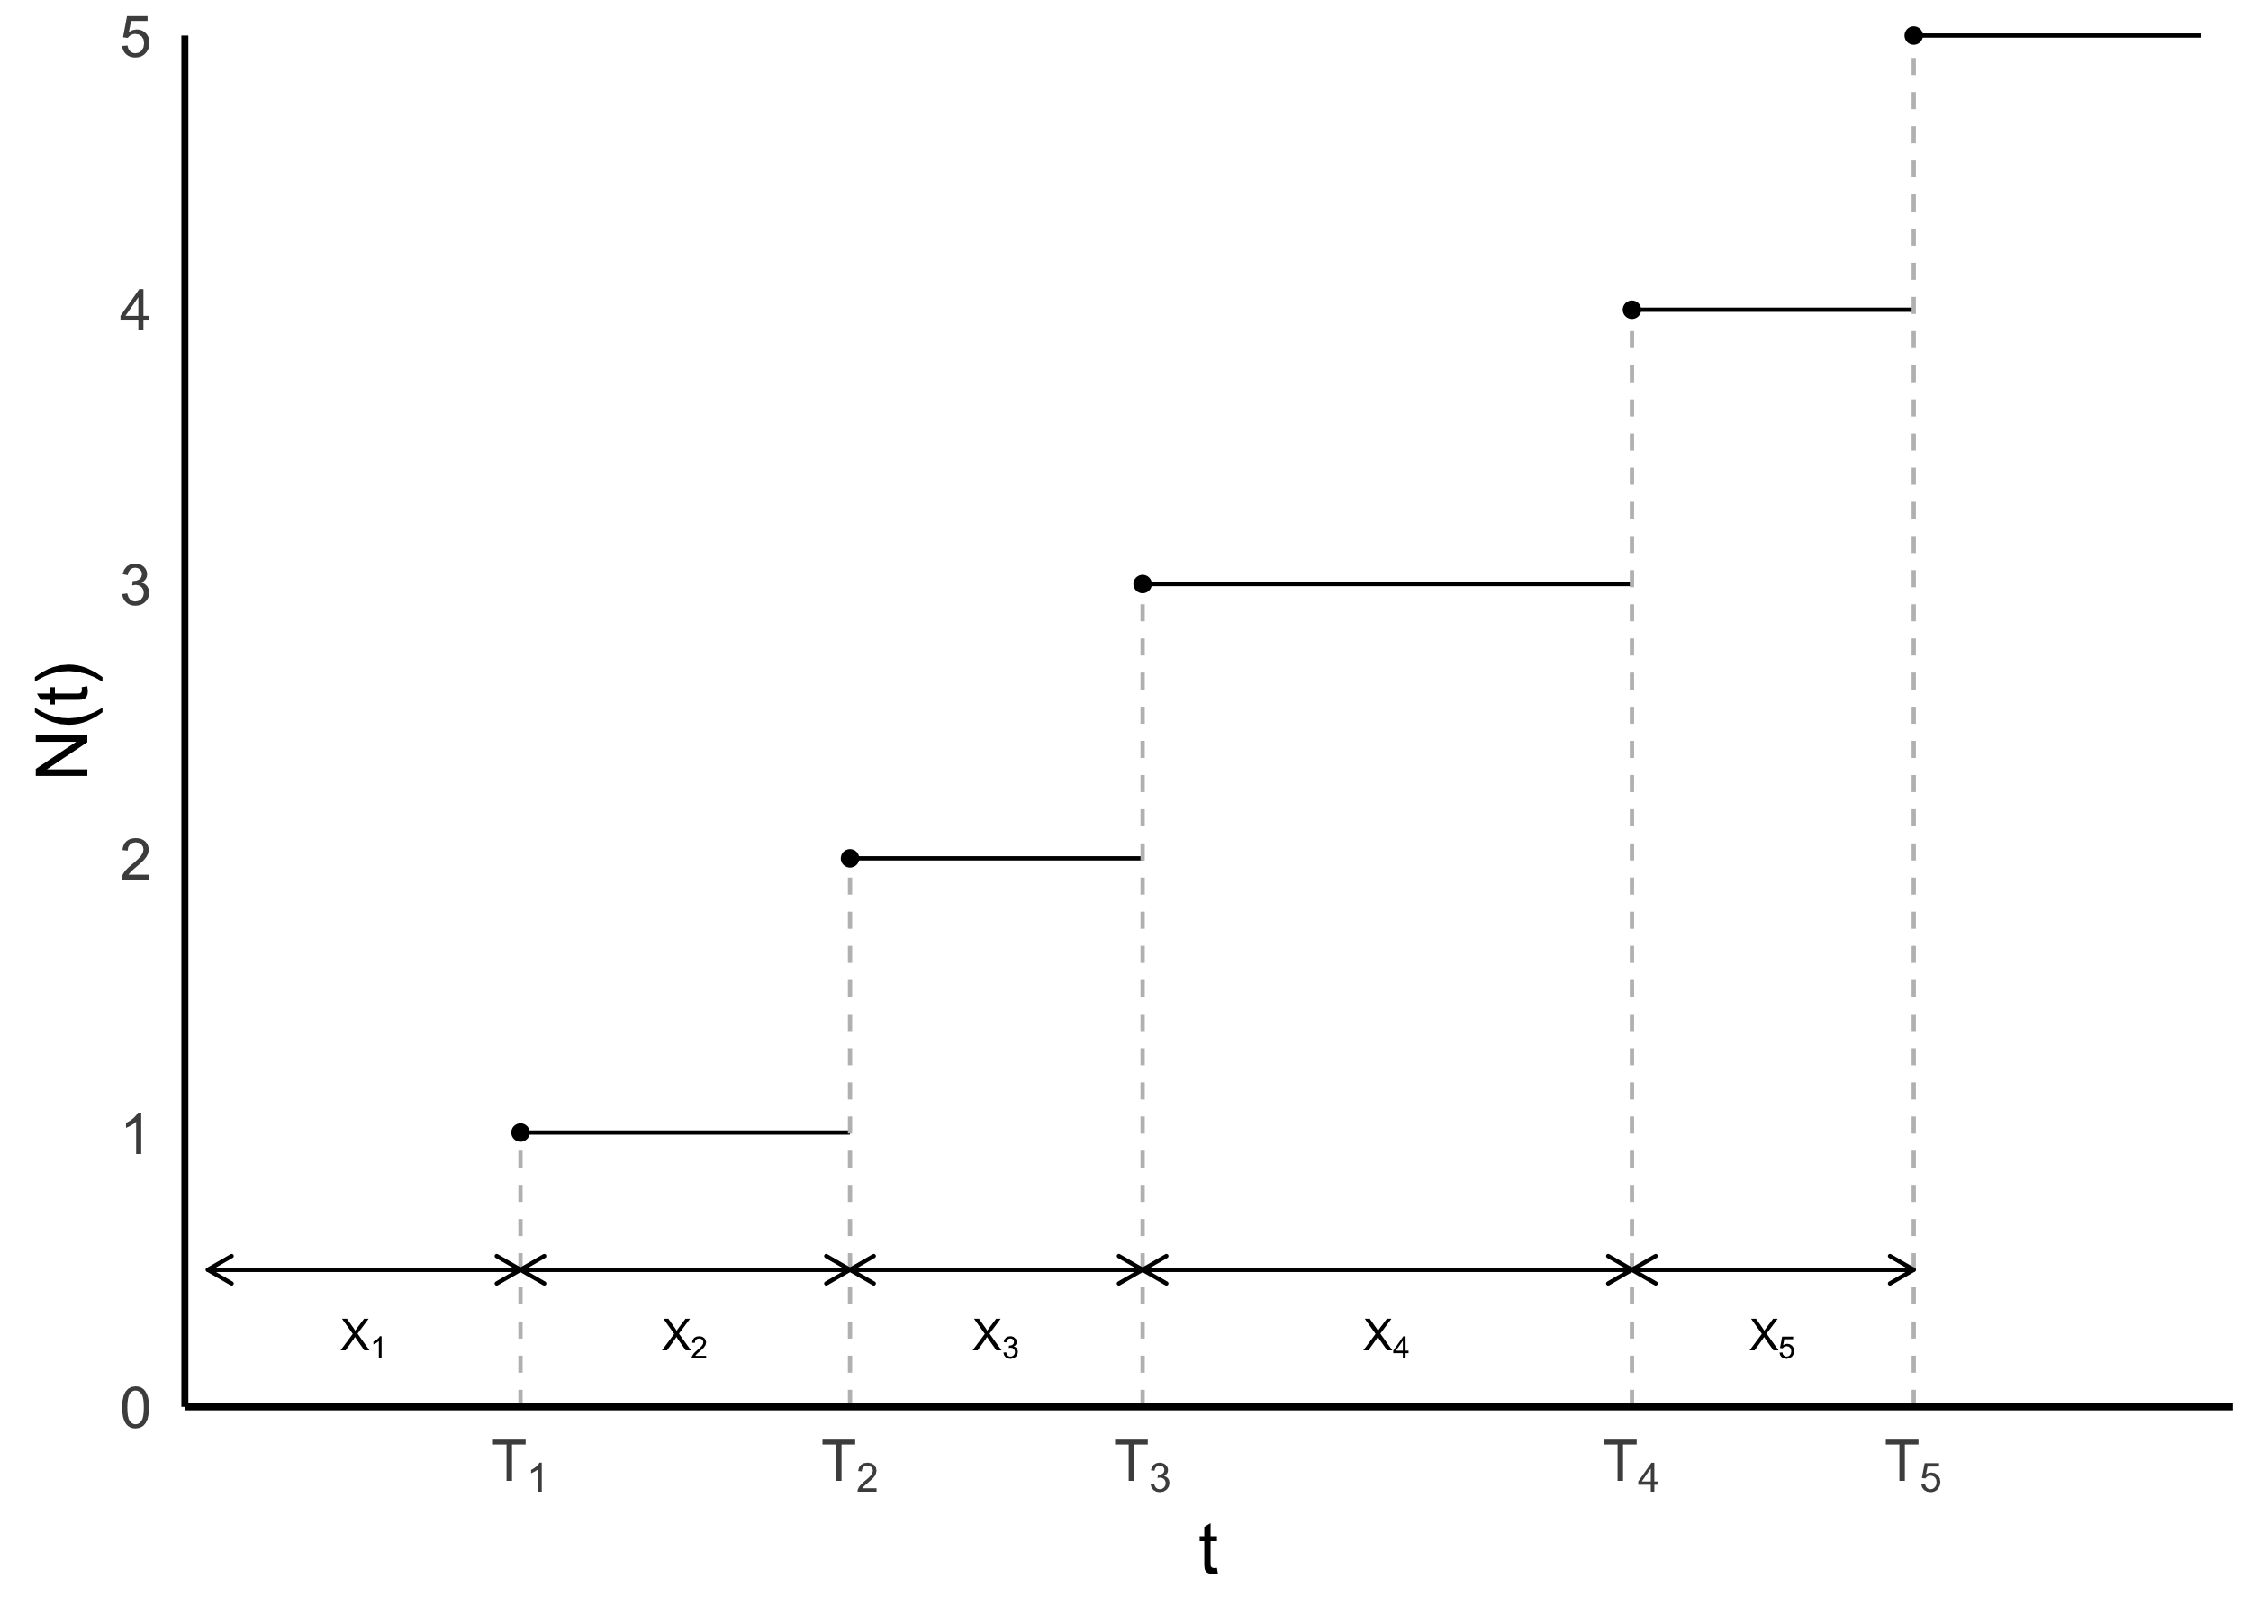
\includegraphics[width=.9\textwidth]{figures/poisson_realization.png}
   \caption{One realization of a Poisson process showing the relationship between $N(t)$, $S_n$, and $X_n$.}
  \label{fig:poisson_realization}
\end{figure}

\begin{theorem}[Poisson Thinning] \label{thm:poisson_thinning}
Let $\{N(t), t \geq 0\}$ be a Poisson process with rate $\lambda$ and $\{X_n\}$ interarrival times.
Assume that for each $X_n$ in the process, we classify as 1 with probability $p$ and 0 with probability $1 - p$.
The set of all 1 classified points is a Poisson process $\{N_1(t), t \geq 0\}$ with rate $p \lambda$.
Similarly the set of all 0 classified points is a Poisson process $\{N_0(t), t \geq 0\}$ with rate $(1 - p) \lambda$.
$\{N_0(t), t \geq 0\}$ and $\{N_1(t), t \geq 0\}$ are also independent.
\end{theorem}

\begin{theorem}[Poisson Superposition] \label{thm:poisson_super}
Let $\{N_{\lambda_1}(t), t \geq 0\}$ and $\{N_{\lambda_2}(t), t \geq 0\}$ be independent Poisson processes with rate $\lambda_1$ and $\lambda_2$ respectively.
Combining the points from each process we get a new Poisson process $\{N(t) = N_{\lambda_1}(t) + N_{\lambda_2}(t), t \geq 0\}$ with rate $\lambda_1 + \lambda_2$.
\end{theorem}

\section{Matrix Exponential}

\begin{defn}[Matrix Exponential]
The matrix exponential of a real or complex $n \times n$ matrix $A$ is defined as
$$
\exp(A) = \sum_{i = 0}^\infty \frac{1}{i!} A^i
$$
where $A^0 = I$, the $n \times n$ identity matrix.
\end{defn}

\begin{theorem} \label{thm:eigen_matrix_exp}
Assume that $A$ is a diagonalizable $n \times n$ matrix with eigenvalues $\lambda_1, \lambda_2, \ldots, \lambda_n$.
Let $A = T \Lambda T^{-1}$ be the eigendecomposition of $A$ where $T$ is the $n \times n$ matrix of the eigenvectors and $\Lambda = \operatorname{diag}(\lambda_1, \ldots, \lambda_n)$.
Then,
\begin{align*}
    \exp(A) &= T \exp(\Lambda) T^{-1}\\
    &= T \operatorname{diag}(\exp(\lambda_1), \ldots, \exp(\lambda_n)) T^{-1}
\end{align*}
\end{theorem}